%% LyX 2.3.3 created this file.  For more info, see http://www.lyx.org/.
%% Do not edit unless you really know what you are doing.
\documentclass[english]{article}
\usepackage[T1]{fontenc}
\usepackage[latin9]{inputenc}
\usepackage{float}
\usepackage{graphicx}

\makeatletter

%%%%%%%%%%%%%%%%%%%%%%%%%%%%%% LyX specific LaTeX commands.
%% Because html converters don't know tabularnewline
\providecommand{\tabularnewline}{\\}

%%%%%%%%%%%%%%%%%%%%%%%%%%%%%% User specified LaTeX commands.
\date{}

\@ifundefined{showcaptionsetup}{}{%
 \PassOptionsToPackage{caption=false}{subfig}}
\usepackage{subfig}
\makeatother

\usepackage{babel}
\begin{document}
\title{CSE 601 - Project 2 - Clustering Algorithms}
\author{Dipack P Panjabi (50291077), Krithika Srinivasan (50290373)}
\maketitle

\section{Overview}

This project focuses on implement 5 different clustering algorithms
- KMeans, Hierarchical Agglomerative clustering with Min approach,
density-based clustering, Gaussian mixture model clustering, and Spectral
clustering. These 5 clustering methods are tested on two provided
datasets, and their results are compared.

We use two external indexes to compare the clustering performance
of these algorithms, with the ground truth clusters - Rand Index,
and Jaccard Coefficient. We also visualise the resultant clusters,
by reducing their dimensions down to 2, using Principal Component
Analysis (PCA).

\section{Implementation}

\subsection{KMeans}

The KMeans algorithm is relatively simple to implement. The algorithm
is as follows:
\begin{enumerate}
\item From the given data, we select $n$ centroids, by selecting the first
$n$ data points, thereby giving us $n$ clusters.
\item We then assign each of the points in the data set to the cluster closest
to it, measured using Euclidean distance.
\item Once we have assigned all the points, we recompute the centroids of
each of the clusters, by averaging the coordinates of all the points
in the cluster.
\item Using the newly computed centroids, we repeat steps 2, and 3, until
we reach a point where the Euclidean distance between the old and
new cluster centroids is below a threshold, or, we have iterated a
enough times over the data set.
\end{enumerate}
\begin{figure}[H]
\subfloat[cho.txt]{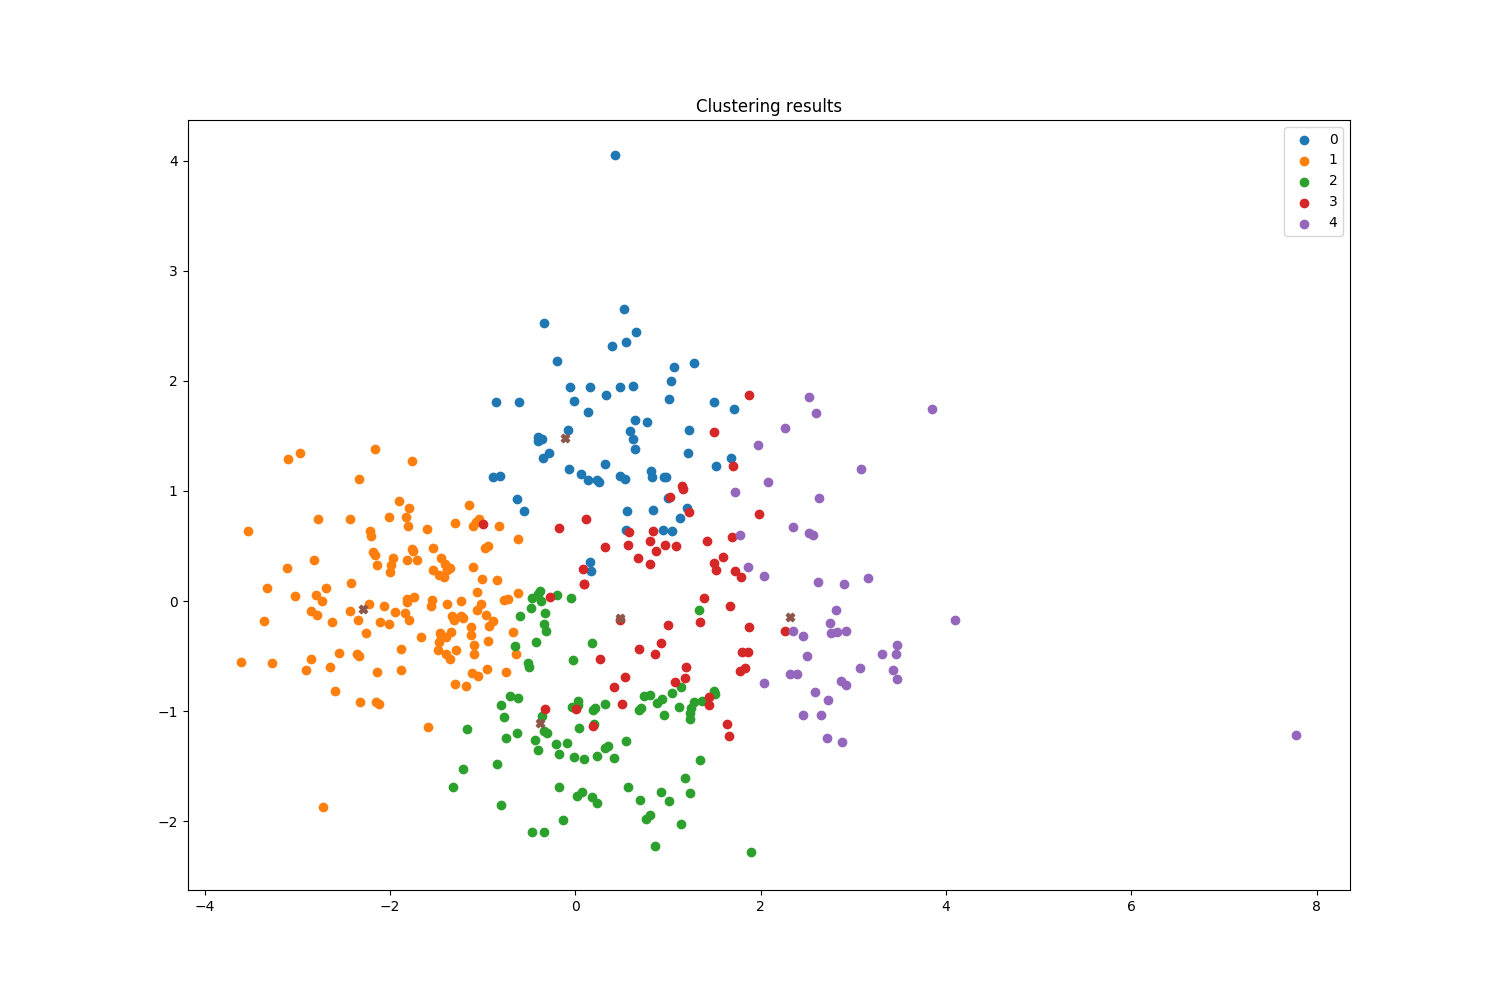
\includegraphics[scale=0.3]{images/cluster_kmeans_cho}

}\hfill{}\subfloat[iyer.txt]{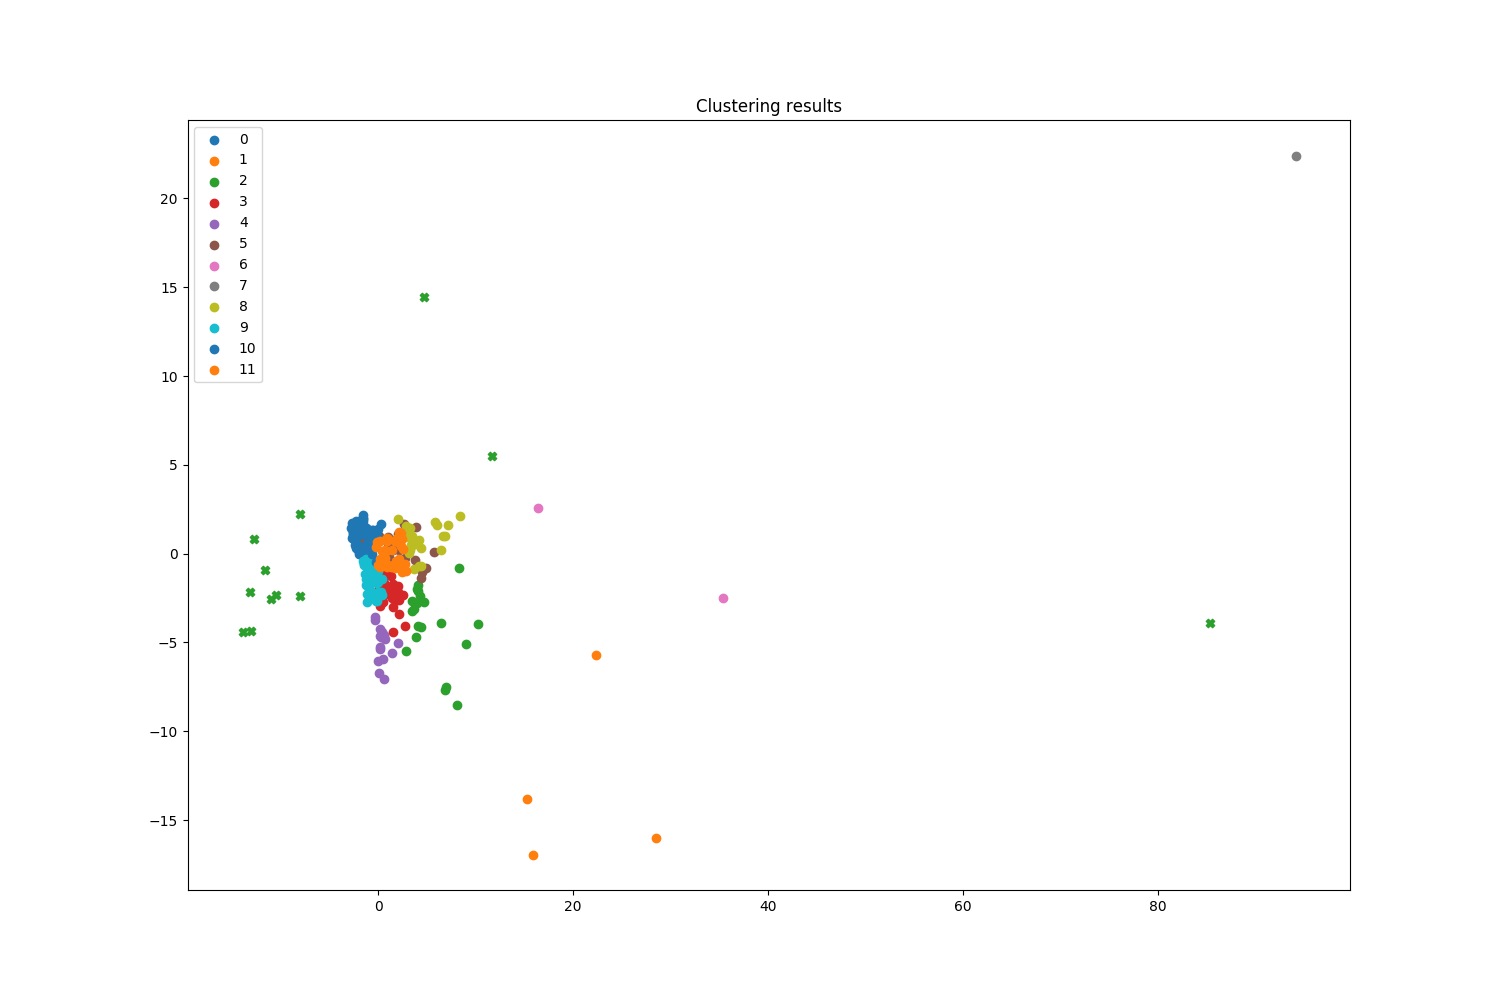
\includegraphics[scale=0.3]{images/cluster_kmeans_iyer}

}

\caption{KMeans clustering results}

\end{figure}

Figure 1 shows us the clusters computed by KMeans for each of the
two data sets. The cluster centroids are denoted as crosses - `x'.

\begin{table}[H]
\begin{tabular}{|c|c|c|}
\hline
Dataset & Rand Index & Jaccard Coefficient\tabularnewline
\hline
\hline
cho.txt & 0.791 & 0.480\tabularnewline
\hline
iyer.txt & 0.786 & 0.0174\tabularnewline
\hline
\end{tabular}

\caption{KMeans clustering external index values}

\end{table}

Table 1 shows us the Rand Index, and Jaccard coefficient values for
the KMeans clusters generated for the two data sets.

From the table, we can see that both the Rand index, and Jaccard coefficient
are higher for the `cho.txt' data set, indicating that that particular
data set is better classified by KMeans. This is also corroborated
by the the data set visualizations in Figure 1, where the clusters
for `iyer.txt' are mostly clumped together, away from the actual data
points. A reason for this poor performance could be the fact that
KMeans has a tough time dealing with non-globular clustered data,
or data that has varying cluster densities.

The advantages of KMeans, on the other hand, are exhibited quite nicely
by its performance on `cho.txt', which seems to be clustered quite
well, owing to the fact that most of the clusters have similar density,
and are spherically shaped in 2 dimensions.

\subsection{Hierarchical Agglomerative Clustering}

The hierarchical agglomerative clustering algorithm is as follows,
\begin{enumerate}
\item Each point in the given data is put into its own cluster, giving us
$n$ clusters for $n$ points.
\item We compute the inter-cluster distances, and use a Min Queue to store
them.
\begin{enumerate}
\item A Min Queue is a type of queue where the cluster pair with the shortest
distance is `popped'
\item The inter-cluster distance is computed by measuring the Euclidean
distance between between the two closest points between the two clusters.
\end{enumerate}
\item Once we have the two closest clusters in the current iteration, we
combine them to form a single cluster, replacing the two clusters,
and compute the inter-cluster distances again.
\item We repeat step 3, until we are left with the number of clusters we
want.
\end{enumerate}
\begin{figure}[H]
\subfloat[cho.txt]{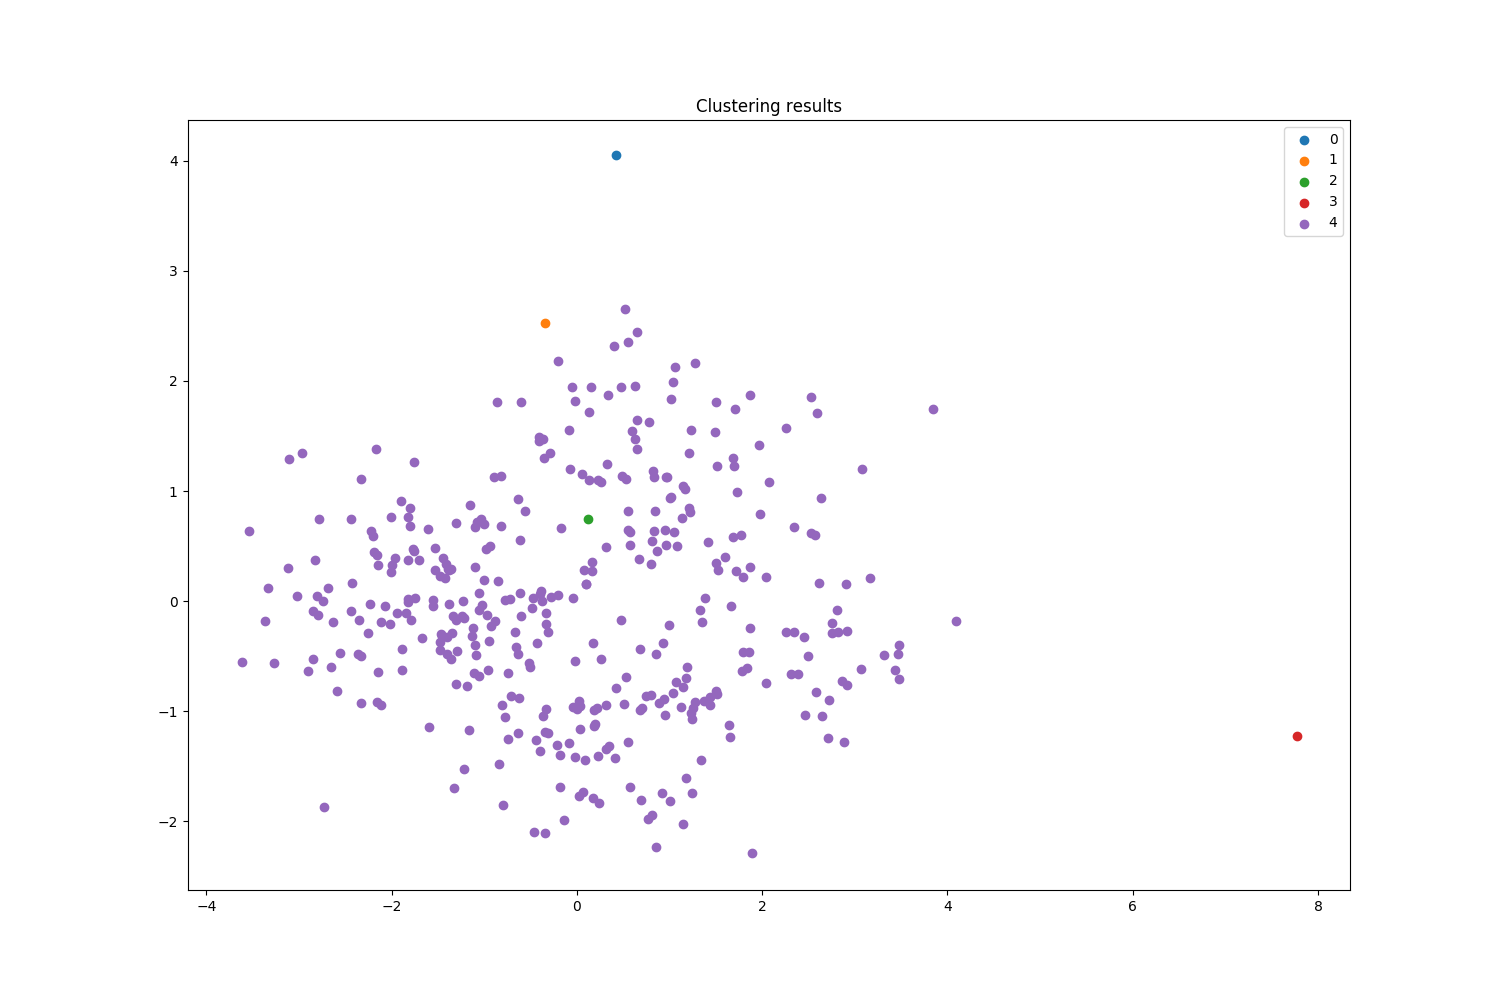
\includegraphics[scale=0.3]{images/cluster_hierarchical_cho}

}\hfill{}\subfloat[iyer.txt]{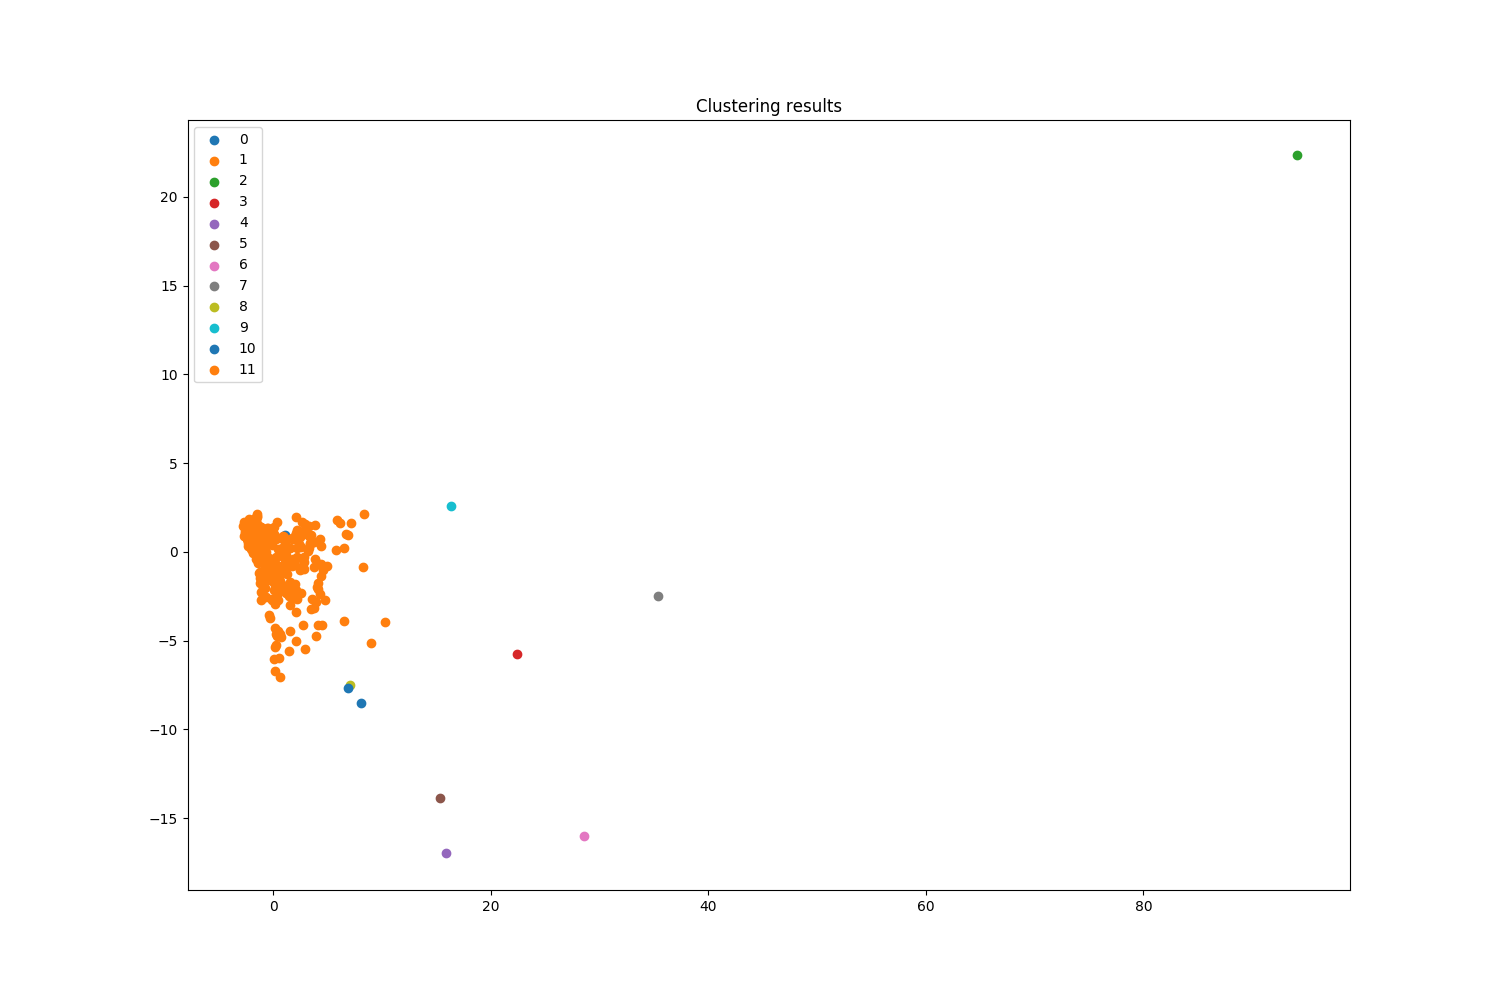
\includegraphics[scale=0.3]{images/cluster_hierarchical_iyer}

}

\caption{Hierarchical agglomerate clustering results}
\end{figure}

Figure 2 shows us the hierarchical agglomerate clusters computed
for each of the two data sets.

\begin{table}[H]
\begin{tabular}{|c|c|c|}
\hline
Dataset & Rand Index & Jaccard Coefficient\tabularnewline
\hline
\hline
cho.txt & 0.238 & 0.0252\tabularnewline
\hline
iyer.txt & 0.192 & 0.00229\tabularnewline
\hline
\end{tabular}

\caption{Hierarchical agglomerate clustering external index values}
\end{table}

Table 2 shows us the Rand Index, and Jaccard coefficient values for
the hierarchical agglomerate clusters generated for the two data
sets.

As the results show us, we get a `mega' cluster for both data sets,
with all the remaining clusters consisting of just a single point
each. The external index results show us that while we do classify
certain points correctly, the overwhelming majority of points are
misclassified. We can conclude that this algorithm performs very poorly,
compared to KMeans, as it is quite sensitive to noise and outlying
points.

An advantage of this clustering technique is the fact that it can
identify and deal with non-elliptical cluster formations.

\subsection{Density-based Clustering}
The DBSCAN algorithm clusters points based on the points' closeness
to each other. The steps to implement it are as follows:
\begin{enumerate}
    \item First, the noise cluster is initialised. Points with an
    insufficient number of points in its neighbourhood will be added
    to this cluster
    \item If a node is unvisited, check whether it contains at least the
    number of points specified in the threshold ($minPts$) in a specified
    radius $\epsilon$
    \item If the number of points in its $\epsilon$ is less than $minPts$,
    then, that point is added to the Noise cluster
    \item If this point does have at least $minPts$ points in its $\epsilon$
    neighbourhood, then a new cluster is created and the point as added as a
    core point of that cluster.
    \item This new point is 'expanded' by visiting its unvisited neighbours.
    If the neighbouring points have at least $minPts$ points in their $\epsilon$
    neighbourhoods and do not already belong to some other cluster, then they
    are added to this cluster as a core point.
    \item Steps 2 to 5 are repeated until all the points in the input data set
    have been visited.
\end{enumerate}
\begin{figure}[H]
\subfloat[cho.txt]{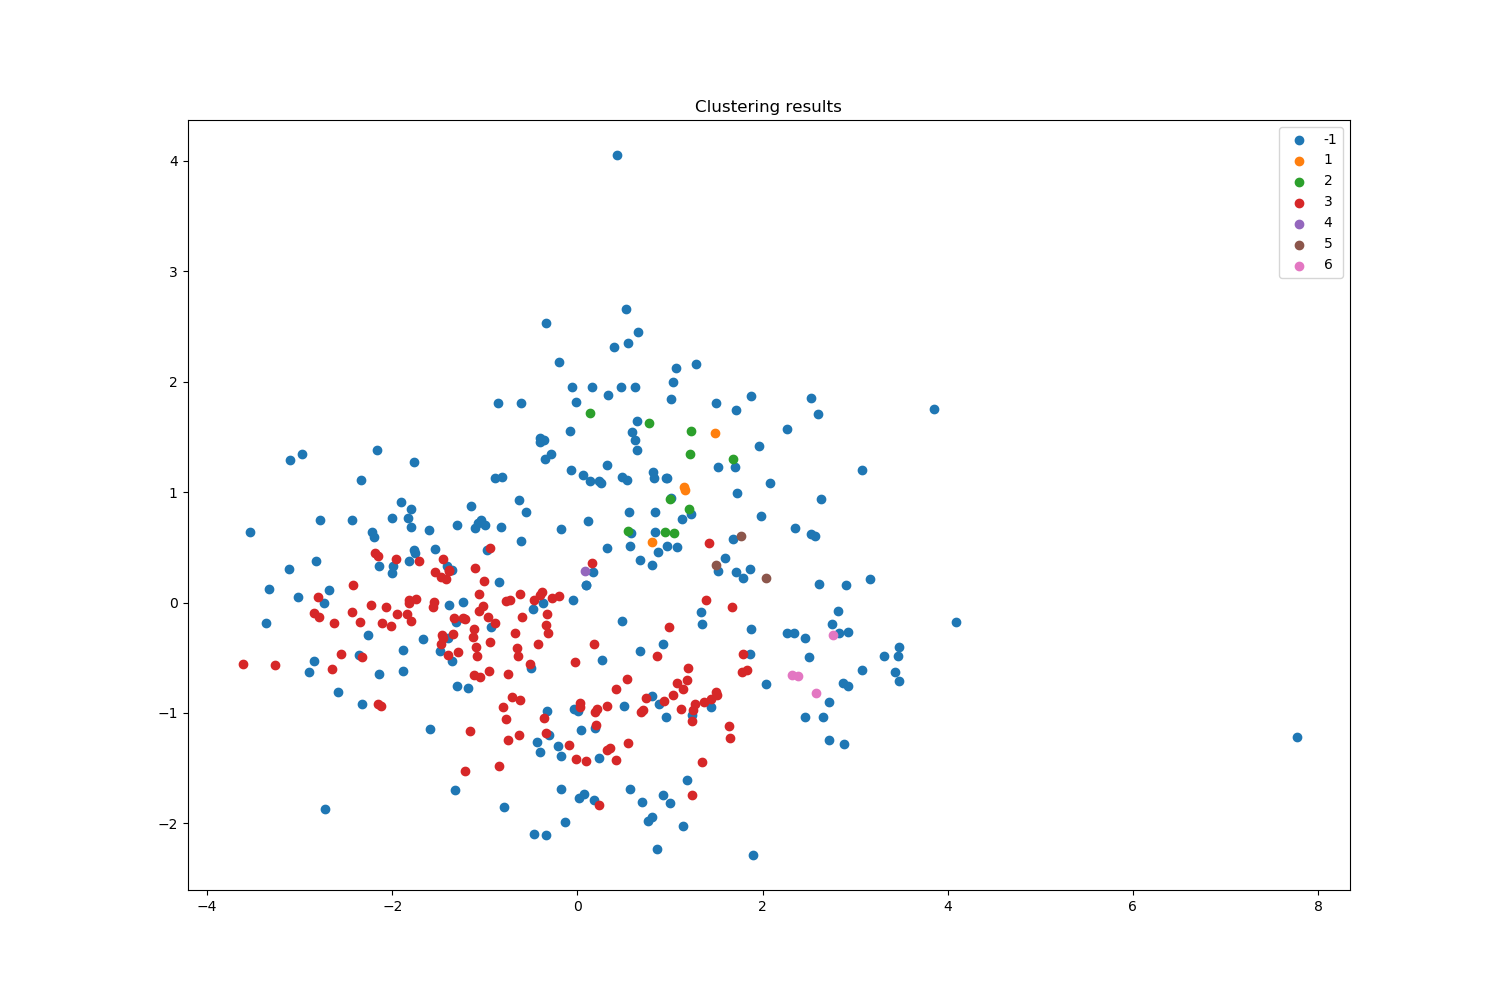
\includegraphics[scale=0.3]{images/cluster_dbscan_computed_cho.png}

}\hfill{}\subfloat[iyer.txt]{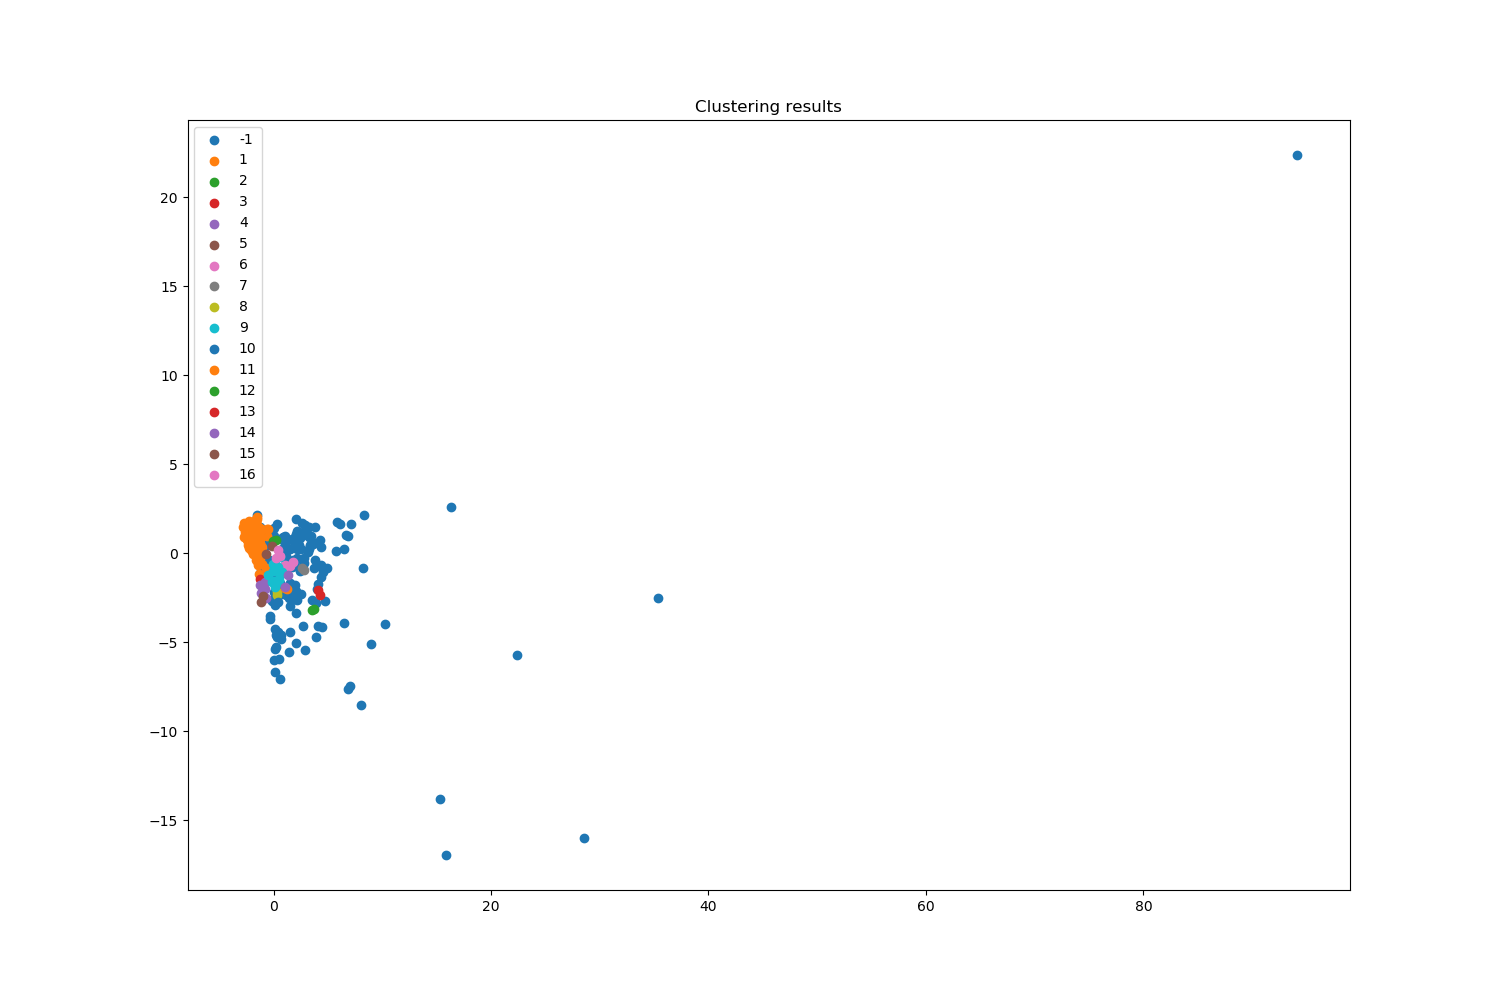
\includegraphics[scale=0.3]{images/cluster_dbscan_computed_iyer.png}

}
\caption{DBSCAN clustering results}
\end{figure}
Figure 3 shows us the DBSCAN clusters computed for each of the two data sets.

\begin{table}[H]
\begin{tabular}{|c|c|c|}
\hline
Dataset & Rand Index & Jaccard Coefficient\tabularnewline
\hline
\hline
cho.txt & 0.535 & 0.200\tabularnewline
\hline
iyer.txt & 0.667 & 0.286\tabularnewline
\hline
\end{tabular}
\caption{DBSCAN clustering external index values}
\end{table}
Table 3 shows us the Rand Index, and Jaccard coefficient values for
the DBSCAN clusters generated for the two data sets.

The outputs of the algorithm in Figure 3 and the external evaluations from
Table 3 highlight the advantages and disadvantages of density-based clustering.
An advantage of DBSCAN is that it intuits cluster shapes based on the distribution
of the points, meaning that we do not specify the number of clusters here. DBSCAN
is useful for identifying irregular cluster shapes since the clustering is done
based on the distribution of points.

DBSCAN also has a good definition for outliers, meaning that their presense does not negatively
impact the output clusters. The algorithm shows a better performance on the Iyer data set
and it is evident that this is because the data points in Iyer are more densely-packed
in a consistent density than in the Cho data set, where different groups of points
have varying densities. This shows us that DBSCAN does not perform as well
with varying densities.

Another point of consideration in the DBSCAN algorithm is that the output clusters are
heavily influenced by the input parameters $\epsilon$ and $minPts$, meaning that these
hyperparameters cannot be selected at random, and have to be selected based on the
layout of the points in the dataset.

\subsection{Gaussian Mixture Models}
Clustering using GMMs makes use of the concept of multimodal Gaussian distributions. The
goal of this kind of clustering is to find the Maximum Likelihood Estimation (MLE) of a
point belonging to a cluster. The steps to perform clustering with GMMs are as follows:

\begin{enumerate}
    \item Get the initial cluster assignment of the data points with K-means clustering
    \item For each cluster obtained by K-means in the first step, calculate the initial
    centroid mean $\mu$, covariance $\sigma$ and the probability of
    selecting the cluster $\pi$.
    \item Once the initial mixture parameters are obtained, Expectation Maximization is
    performed to optimise the cluster assignment.
    \begin{enumerate}
        \item In the expectation step, the points are reassigned to clusters and the
        weight of the probability of a point being assigned membership in a cluster
        is noted
        \item In the maximization step, this weight or expected value is used to update
        $\mu$, $\sigma$ and $\pi$
    \end{enumerate}
    \item The updated $\mu$, $\sigma$ and $\pi$ are used in the calculation of the loss
    function, which here is log-likelihood. Expectation maximization is repeated until
    it converges, i.e, there is no/negligible change in successive iterations
    \item The assigned cluster for a point is the cluster with the highest weight for
    membership
\end{enumerate}
Table 4 shows us the Rand Index, and Jaccard coefficient values for
the GMM clusters generated for the two data sets.
\begin{table}[H]
\begin{tabular}{|c|c|c|}
\hline
Dataset & Rand Index & Jaccard Coefficient\tabularnewline
\hline
\hline
cho.txt & 0.777 & 0.453\tabularnewline
\hline
iyer.txt & 0.741 & 0.006\tabularnewline
\hline
\end{tabular}
\caption{GMM clustering external index values}
\end{table}
Figure 4 shows us the GMM clusters computed for each of the two data sets. We can see that it
performs well on the Cho dataset and fairly well on the Iyer dataset. GMM is posited as a
direct improvement to the K-means algorithm. This is seen in how it can use K-means to obtain
an initial result and then improve on it (although the initial result need not be obtained only
by K-means). Its main advantage over K-means is that since the method of assigning clusters is
based on probability distributions, it can detect clusters of irregular shapes. Another advantage
of GMM-based clustering is that if one chooses to, the concept of overlaps between clusters can
be taken into account. Unlike DBSCAN, varying densities in terms of distribution will not
negatively impact the output.

However, as with K-means, it is important to select good initial centers, as random assignment
may lead to sub-optimal results. Since it is a probabilistic method, there can be issues of
overfitting where smaller nuances of the data might not be picked up on. And as with DBSCAN,
the type of distribution selected greatly affects the quality of the output obtained
\begin{figure}[H]
\subfloat[cho.txt]{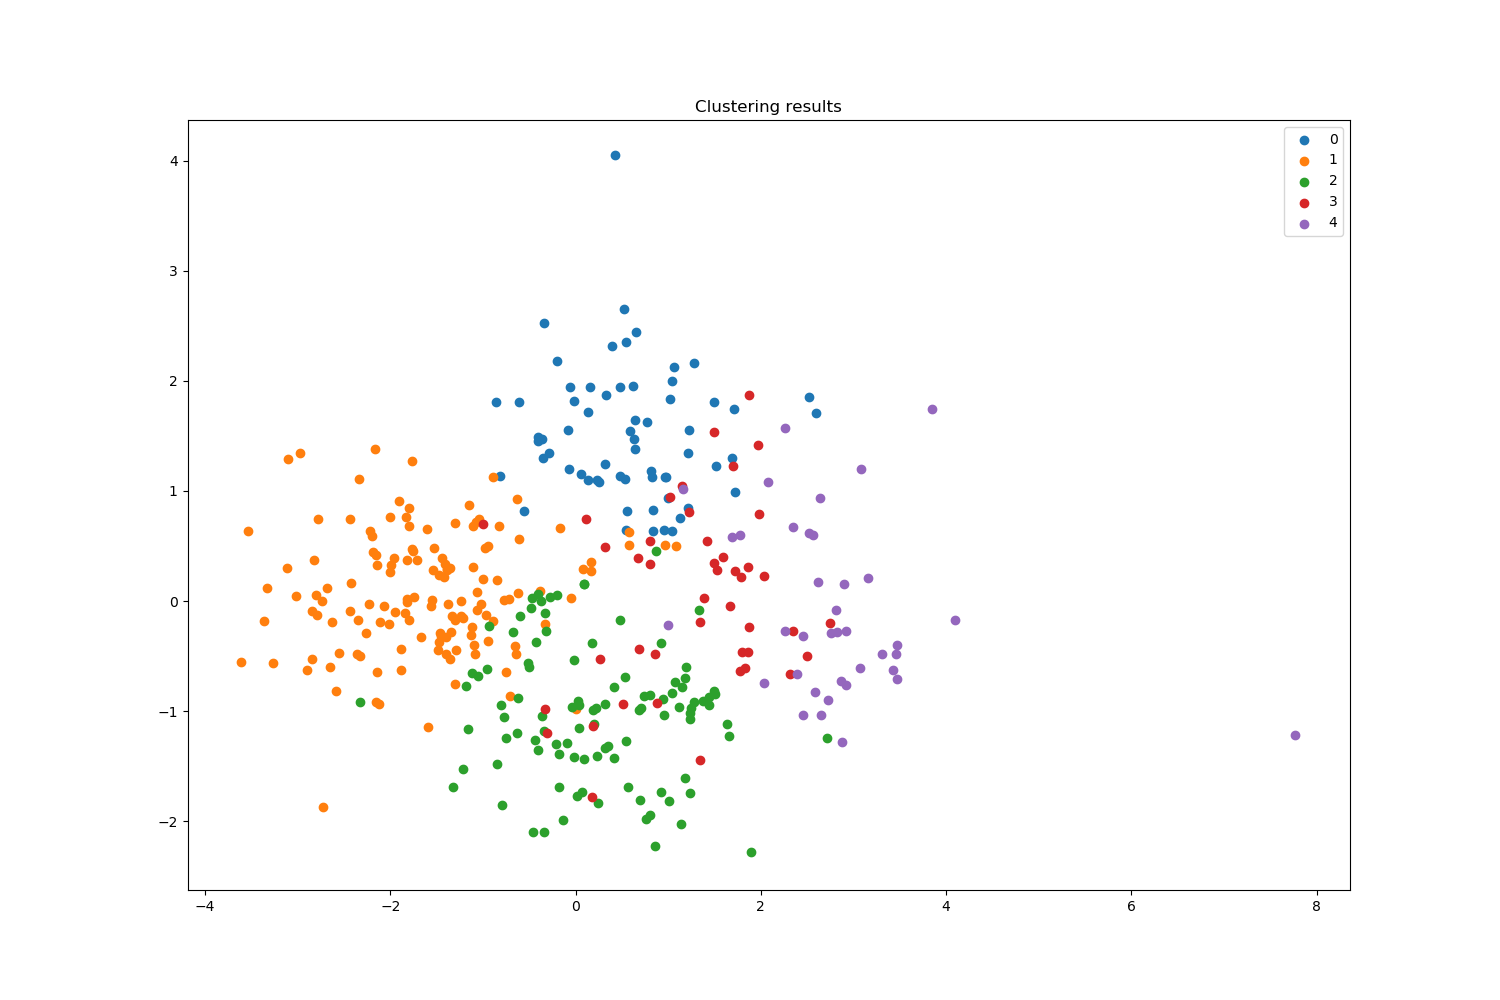
\includegraphics[scale=0.3]{images/cluster_gmm_computed_cho.png}

}\hfill{}\subfloat[iyer.txt]{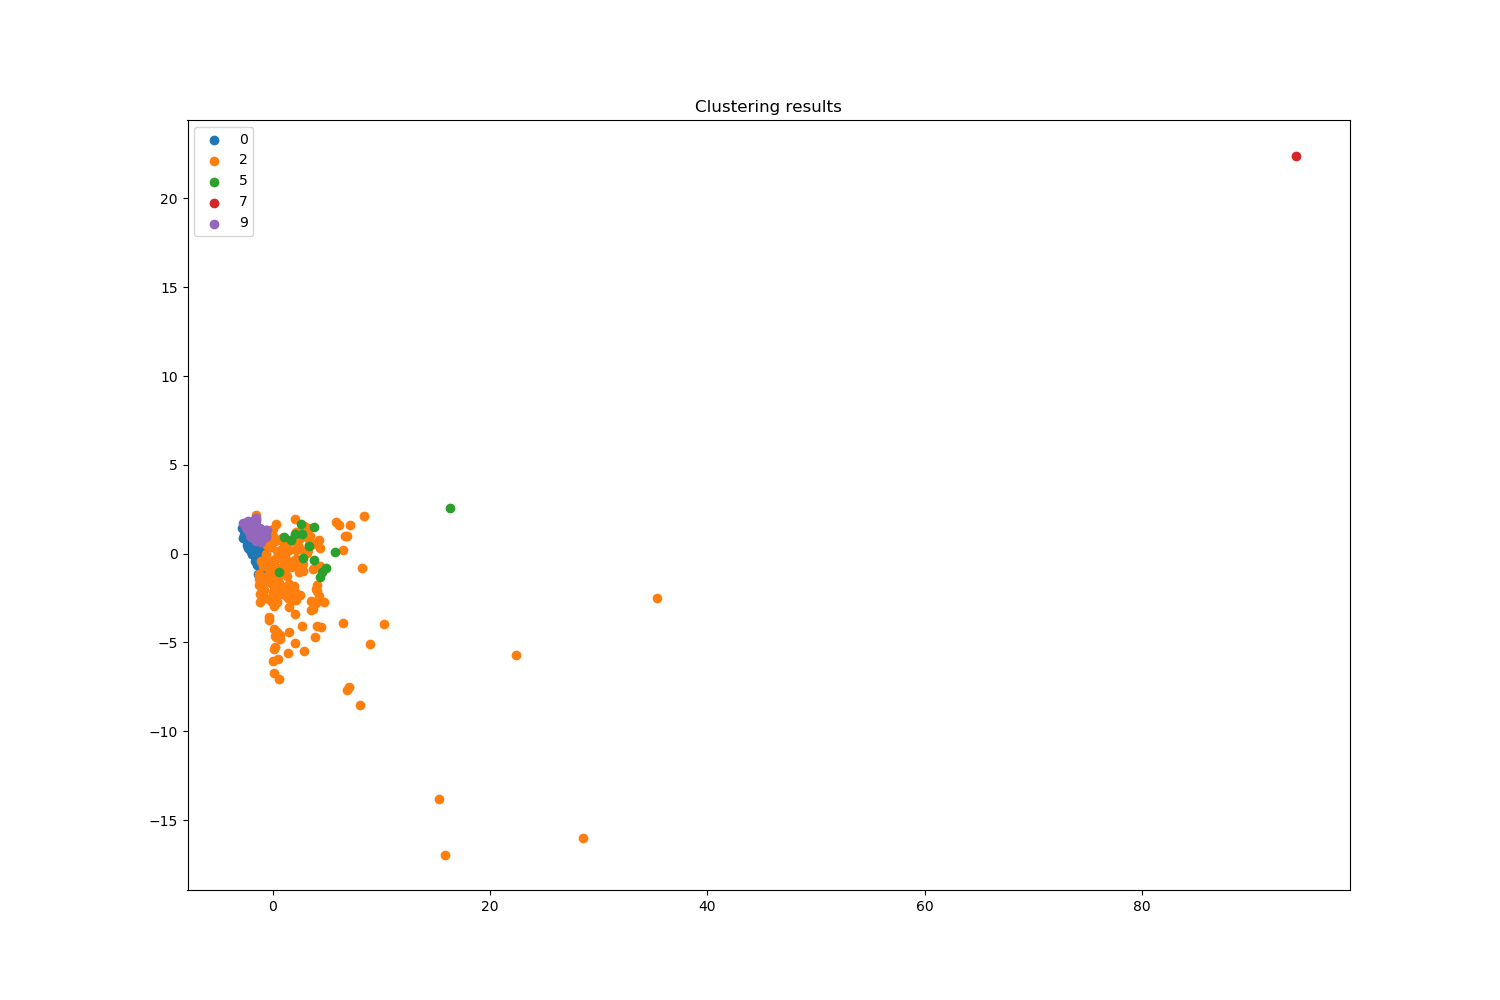
\includegraphics[scale=0.3]{images/cluster_gmm_computed_iyer.png}

}
\caption{GMM clustering results}
\end{figure}

\subsection{Spectral Clustering}
Spectral clustering applies the concept of graph partitioning to clustering data points. The
following are the steps to perform graph partitioning:
\begin{enumerate}
    \item Convert the input data into a fully-connected graph. The edge weights represent the similarity
    of the pair of points, here calculated by the Gaussian kernel. This can be represented as an
    adjacency matrix $W$.
    \item Calculate the degree of each vertex in $W$ and represent this as a degree matrix $D$
    \item Using $W$ and $D$, the graph Laplacian $L$ is calculated. In the unnormalized form,
    it can be calculated as $L = D - W$.
    \item We now calculate the eigenvectors and eigenvalues for the graph Laplacian. This is done
    to perform graph partitioning in the case of multiple clusters efficiently.
    \item For a data set with $n$ items, if the dataset is to be clustered into $k$ clusters, we
    select the eigenvectors for the smallest $k$ eigenvalues to obtain a $n * k$ matrix
    \item K-means clustering is performed on the $n * k$ matrix. The cluster assignment for row $n$
    of this matrix is the cluster assignment for the corresponding row $n$ in the input data set
\end{enumerate}
\begin{table}[H]
\begin{tabular}{|c|c|c|}
\hline
Dataset & Rand Index & Jaccard Coefficient\tabularnewline
\hline
\hline
cho.txt & 0.737 & 0.368\tabularnewline
\hline
iyer.txt & 0.731 & 0.131\tabularnewline
\hline
\end{tabular}
\caption{Spectral clustering external index values}
\end{table}
Table 5 shows us the Rand Index, and Jaccard coefficient values for
the Spectral clusters generated for the two data sets.
\begin{figure}[H]
\subfloat[cho.txt]{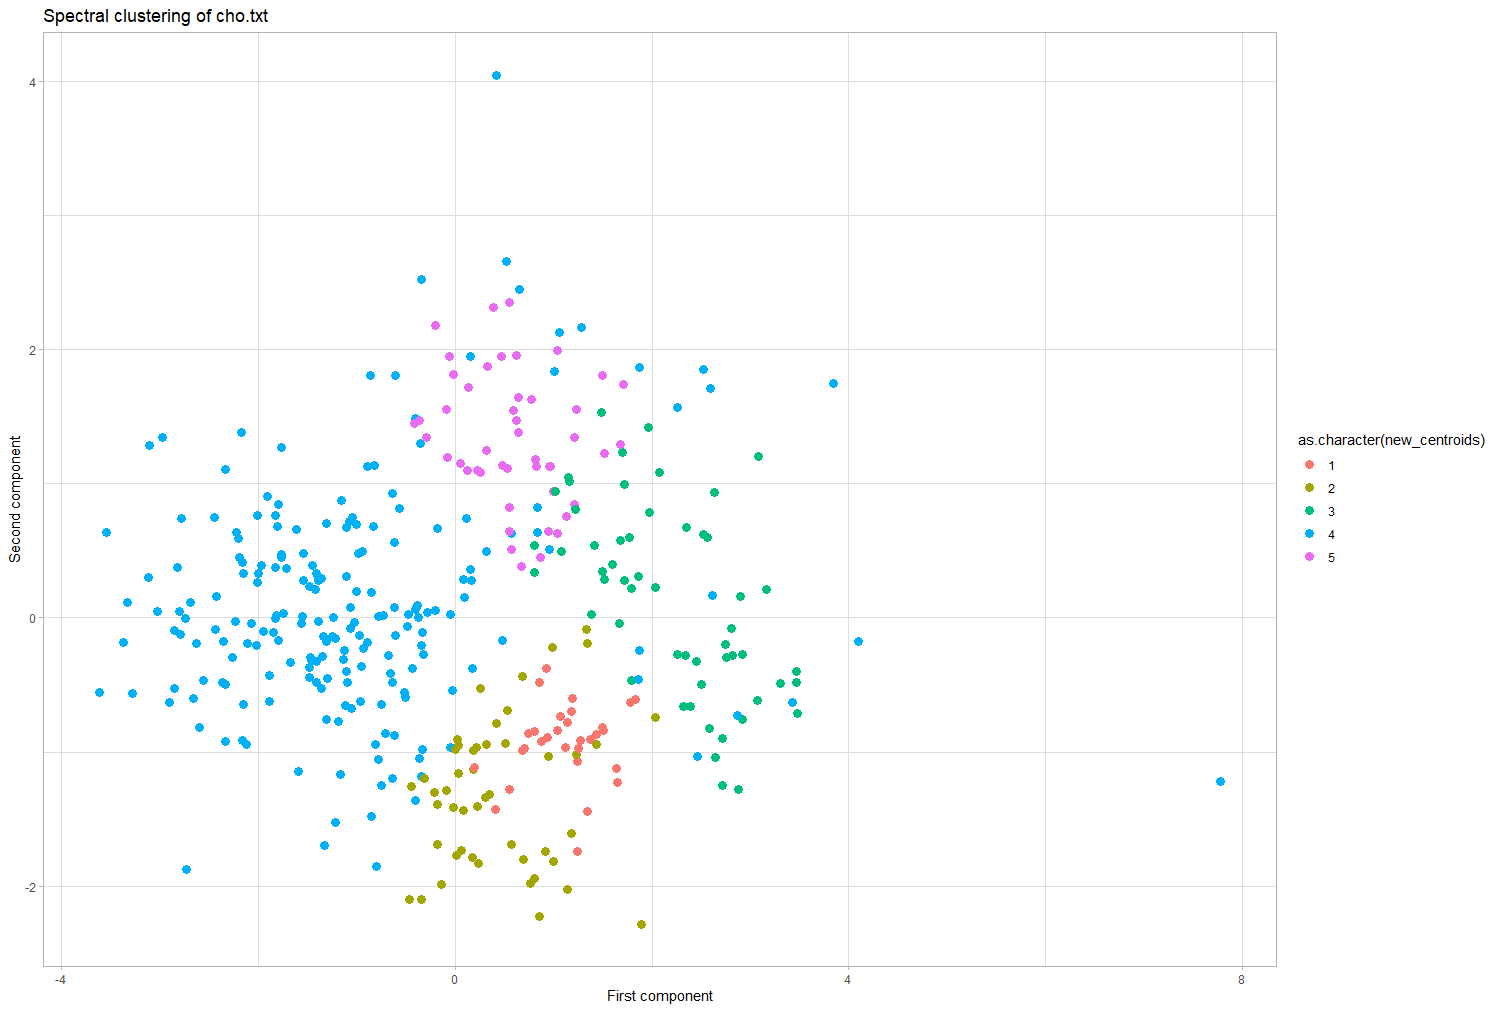
\includegraphics[scale=0.3]{images/cluster_spectral_cho.png}

}\vfill{}\subfloat[iyer.txt]{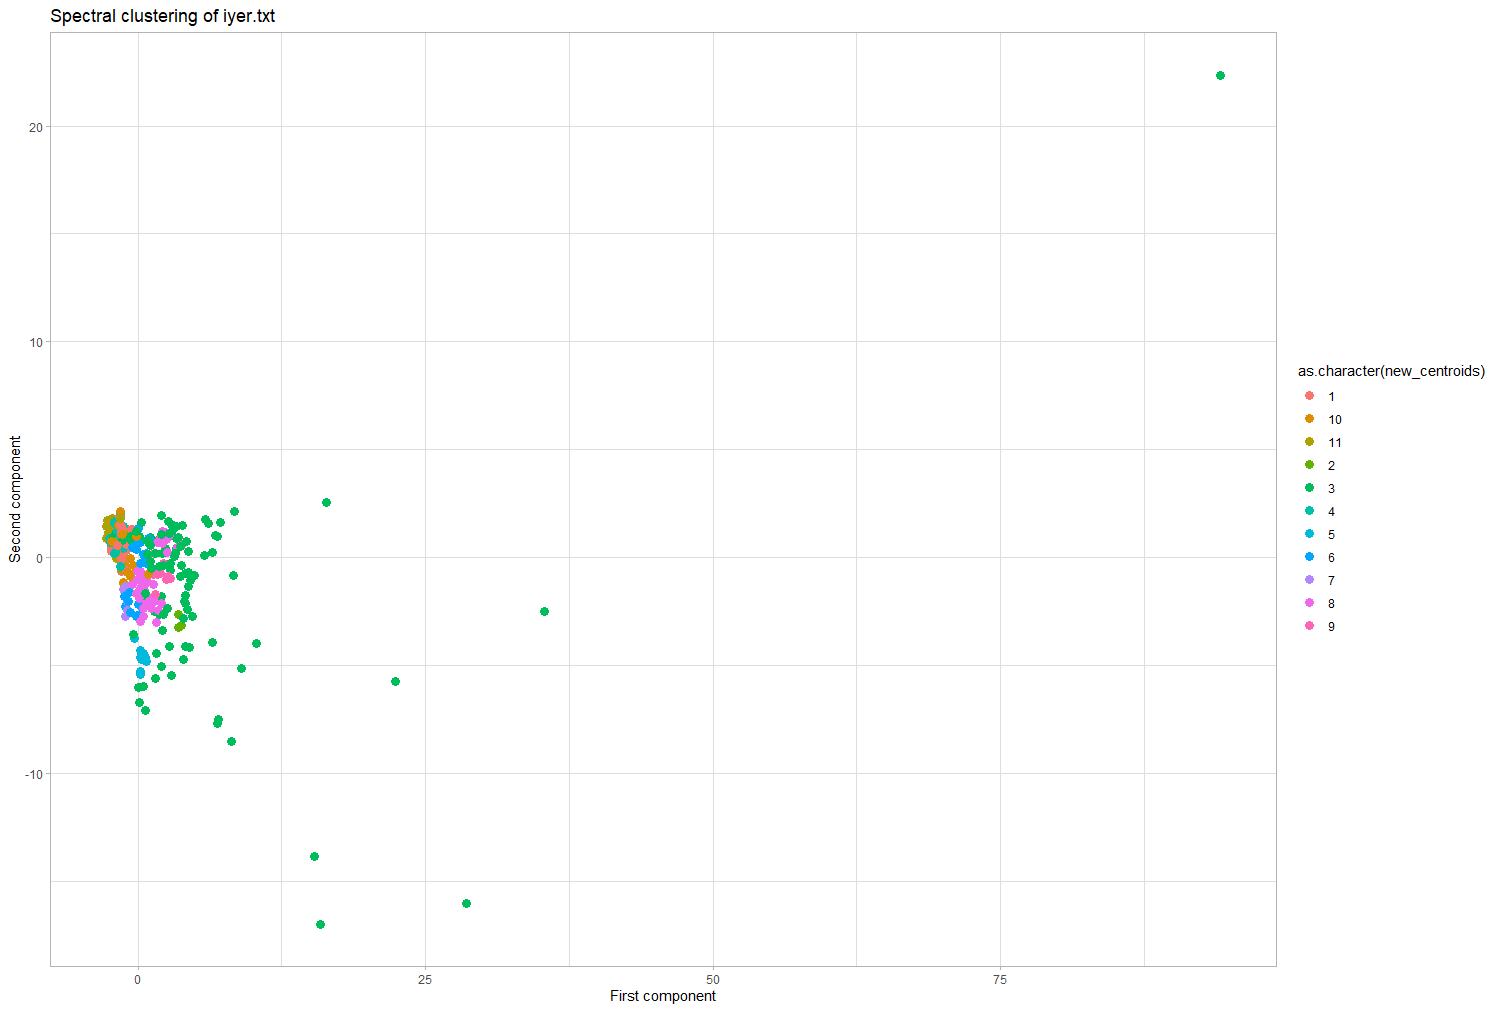
\includegraphics[scale=0.3]{images/cluster_spectral_iyer.png}
}
\caption{Spectral clustering results}
\end{figure}
Figure 5 shows us the Spectral clusters computed for each of the two data sets. We can see both empirically
from Figure 5 and the values from Table 5 that Spectral clustering produces good results for both datasets,
meaning that the distribution of the data points is not as big a consideration for this method. In fact,
spectral clustering's distinguishing characteristic is that it has a solid foundation in mathematics and
graph theory. This means that spectral clustering performs consistently well for different types of input
data, as seen with its high Rand indices for both the input data sets.

One point of consideration is that the metric used to establish similarity between points can affect the
output, e.g. using K-nearest neighbours versus the Gaussian kernel can produce different results.
Even within the similarity measures, Spectral clustering is sensitive to parameters. In our
implementation with the Gaussian kernel, changing the kernel bandwidth $\sigma$ can dramatically alter the
cluster assignment and its quality.

\section{Conclusion}
Clustering algorithms are a way to group points in a data set without any prior labels
pertaining to groups. For this project, we implemented five different types of clustering
algorithms: K-means, hierarchical agglomerate, DBSCAN, GMM and Spectral clustering. We
observed the outputs these algorithms produce by plotting the assignments on two-
dimensional representations of the data sets and evaluated the correctness of the
cluster assignment with the Rand Index and Jaccard coefficients. Using these plots
and measures, we were able to observe the strengths and weaknesses of each clustering
algorithm and understand the situations for each of these algorithms would be
suitable.
\end{document}
